\chapter{Aspectos Generales}
\section{Aspectos Generales}
\subsection{Descripción del Problema}
Uno de los sentidos más importantes de los seres humanos es la visión. Ésta es empleada para obtener la información visual del entorno físico. Según Aristóteles, “Visión es saber que hay y donde mediante la vista”. De hecho, se calcula que más del 75\% de las tareas del cerebro son empleadas en el análisis de la información visual. El refrán popular de “Una imagen vale más que mil palabras” tiene mucho que ver con los aspectos cognitivos de la especie humana. Casi todas las disciplinas científicas emplean utillajes gráficos para transmitir conocimiento\footnote[1]{Visión Humana, fuente: Sistemas Adaptativos y Bioinspirados en Inteligencia Artificial\href{http://sabia.tic.udc.es/}{(S.A.B.I.A.)}}.

Uno de los más grandes concursos a nivel mundial en clasificación de imágenes reporta que las técnicas tradicionales (como las técnicas de extracción de características en imágenes estáticas: \textit{Principal component analysis} (PCA), \textit{Edges detector}, \textit{Gabor waveled}; Video: PCA, \textit{Discrete cosine transform} (DCT), \textit{optical flow} e \textit{image difference}) están siendo superadas por técnicas de \textit{Deep Learning} basadas en el proceso cerebral humano. Dicho éxito se debe a que las técnicas tradiciones requieren de un ambiente controlado y no son tolerables a cambios como: traslación, rotación y escalado, por otro lado las técnicas de \textit{Deep Learning} demustran ser mas robustas y efectivas frente a estos tipos de cambios\footnote[2]{\textit{Deep Learning} vs. \textit{Machine Learning} fuente: \href{http://www.image-net.org/}{Analytics Vidhya}}.
	
Diversas actividades cotidianas necesitan del reconocimiento de imágenes, tal es el caso del reconocimiento de expresiones faciales, que en los últimos años se ha convertido en una de las tareas más estudiadas por investigadores en todo el mundo, con el fin de alcanzar un margen de error minimo para posteriormente centrarse en el desarrollo de aplicaciones en distintos campos, como: estudio de marketing, interacción hombre-máquina, psicología y análisis educativo \footnote[3]{Las expresiones faciales de las emociones, historia y aplicaciones, fuente: \href{http://medina-psicologia.ugr.es/cienciacognitiva/?p=664}{Ciencia Cognitiva}}, las cuales han sido abordada por diferentes técnicas tradicionales no obteniendo los resultados prometedores en imagenes reales que contienen distintos tipos de variaciones (mencionados en el parrafo anterior) limitando asi la implementacion y desarrollo de aplicaciones utiles para el bien comun (aplicaciones antes mencionadas).

\subsection{Identificación del Problema}
Las técnicas tradicionales para el reconocimiento de expresiones faciales usadas en la actualidad necesitan de un ambiente controlado (iluminacion constante, alta calidad de imagen, poco ruido, imagen sin oclusión), y no son tolerables a cambios como rotación, traslación, escalado, limitando asi la creacion de aplicaciones con imagenes del mundo real(imagenes obtenidas a partir de camaras de seguridad) . Por lo que hay la necesidad de usar nuevas técnicas del estado del arte que nos permitiran obtener mejores resultados superando asi la limitacion antes mencionada.

\section{Antecedentes}
Se muestra una lista de trabajos resaltantes que hacen uso de tecnicas de \textit{Deep Learning}, los cuales sirvieron de inspiración y fuente de información valiosa en el desarrollo de este trabajo. Tambien se presentan trabajos dedicados al reconocimiento de expresiones faciales utilizando tecnicas tradicionales de vision por computador y \textit{machine learning}.

\vspace{1cm}
\textbf{“Gradient-Based Learning Applied to Document Recognition” \cite{2lecun1998gradient}}\\
\textbf{Descripción:}\\

\begin{itemize}
\item Este proyecto muestra uno de los inicios en lo que respecta al aprendizaje profundo con Redes Neuronales Convolucionales
\item Este proyecto utiliza la data set MNIST, la función de activación no lineal tanh(x) y el promedio aritmético para la parte del Submuestreo y obtuvo un 99.3% de precisión.
\item Este proyecto utiliza un paradigma de aprendizaje denominada “Redes transformadoras de gráfico”, tal sistema permite entrenar varios módulos basado en el gradiente, con el fin de minimizar la medida del rendimiento global.
\end{itemize}
\textbf{Objetivo:} Reconocer documentos manuscritos\\
\textbf{Conclusión:} La utilización de Gradient Based learning permitió alcanzar altos niveles de precisión en el reconocimiento de documentos manuscritos, dando más relevancia al Deep Learning.\\


\textbf{“Traffic Sign Recognition with Multi-Scale Convolutional Networks” \cite{12sermanet2011traffic}}\\
\textbf{Descripción:}\\

\begin{itemize}
\item Este trabajo se hizo como parte de la competencia GTSRB.
\item En este trabajo se aplican Redes Neuronales Convolucionales en la tarea de clasificación de señales de tráfico, estas Redes Neuronales Convolucionales aprenden características en todos los niveles de su arquitectura.
\item Este trabajo produjo una precisión de 98.31\% durante la competición estando por debajo con 0.53\% de diferencia respecto al rendimiento humano que es del 98.81\%.
\end{itemize}
\textbf{Objetivo:} Reconocer señales de transito\\
\textbf{Conclusión:} Las Redes Convolucionales Multi - Escalas son mejores en el reconocimiento de señales de transito a comparación con la mayoria de técnicas tradicionales\\




\textbf{“Multi-column Deep Neural Networks for Image Classification” \cite{4ciregan2012multi}}\\
\textbf{Descripción:}\\

\begin{itemize}
\item Este paper menciona que los métodos tradicionales de visión por ordenador y Machine Learning no podían igualar el rendimiento humano en tareas tales como el reconocimiento de dígitos escritos a mano o señales de tráfico. 
\item Este paper menciona que se crean varias columnas neuronales profundas, que se convierten en expertos en áreas específicas de las entradas pre-procesadas. Este método es el primero en lograr un rendimiento casi humano. 
\item Este paper menciona que se crean varias columnas neuronales profundas, que se convierten en expertos en áreas específicas de las entradas pre-procesadas. Este método es el primero en lograr un rendimiento casi humano. 
\item En este proyecto logra una precisión del 99.46\% en el reconocimiento de señales de tráfico superando a su predecesor por un 0.24\% y logrando un rendimiento superior al humano por 0.62\%.
\end{itemize}
\textbf{Objetivo:} Evaluar el rendimiento de las Redes Neuronales Profundas Multi-Columnas en la clasificación de imágenes.\\
\textbf{Conclusión:} Las Redes Convolucionales Multi - Escalas son mejores en el reconocimiento de señales de transito a comparación con la mayoria de técnicas tradicionales.\\


\textbf{“ImageNet Clasificación with Deep Convolutional Neuronal Networks” \cite{8krizhevsky2012imagenet}}\\
\textbf{Descripción:}\\

\begin{itemize}
\item En este proyecto se unas ImageNet, que es una data set compuesto de más de 100.000 categorías con cerca de 1.2TB de iimágenes, desarrollada por el laboratorio de visión de la Universidad de Stanford.
\item Este proyecto crea un modelo basado en los trabajos desarrollados hasta ese momento referente a Redes Neuronales Convolucionales logrando bajar el error de $\pm$ 25\% a $\pm$ 15\%. Su modelo consistía en 650K neuronas, 832M de sinapsis y 60M de parámetros. El entrenamiento de su modelo se realizó con 2 GPU’s durante el tiempo de 1 semana.
\end{itemize}
\textbf{Objetivo:} Clasificación de imágenes de la base de datos ImageNet en más de 1000 categorías, utilizando Redes Neuronales Convolucionales.\\
\textbf{Conclusión:} Las Redes Neuronales Convolucionales logran alto nivel de precisión gracias a la gran cantidad de datos en la fase de entrenamiento y a la utilización de GPU's\\




\textbf{“Teaching Deep Convolutional Neural Network to Play Go” \cite{13clark2015training}}\\
\textbf{Descripción:}\\

\begin{itemize}
\item Este trabajo logra desarrollar una Red Neuronal Convolucional, que es capaz de lograr precisión de predicción de una posición de una pieza de 41.1\% y 44.4\% en los diferentes conjuntos de datos de Go superando anteriores técnicas del estado del arte en esta tarea por márgenes significativos.
\end{itemize}
\textbf{Objetivo:} Crear un programa capaz de jugar a Go mediante Deep Learning.\\
\textbf{Conclusión:} Las Redes Neuronales Convolucionales no solo sirven para la visión por computador, sino también son muy útiles para la teoría de juegos.\\


\section{Objetivos}
\subsection{Objetivo General}
Desarrollar una arquitectura de Red Neuronal Convolucional que sea capaz de obtener niveles de precision confiables (con un minimo margen de error) en el reconocimiento de expresiones faciales, permitiendo asi contribuir en el desarrollo de futuras aplicaciones del mundo real que sirvan para el beneficio de la sociedad.
\subsection{Objetivos Específicos}
\begin{itemize}
\item Selección de las bases de datos de expresiones faciales y transformación de datos a un formato estandar para su posterior utilizacion.
\item Investigar los filtros de convolucion para la correcta seleccion de los parametros.
\item Investigar la funcion de submuestreo para la correcta selección de los parametros. 
\item Investigar las funciones de activación y funciones de normalizacion para la correcta selección de los parametros.
\item Diseñar la arquitectura propuesta(configuracion de parametros, numero de capas y funciones de activacion y normalizacion), basandonos en los objetivos previos.
\item Entrenar la arquitectura propuesta.	
\item Evaluar el modelo creado a partir de la arquitectura propuesta.
\item Analizar e interpretar los resultados
\end{itemize}

\section{Alcances}
En este trabajo de investigacion se lograron los siguientes alcances.

\begin{itemize}
\item Se propuso una nueva arquitectura para el reconocimiento de expresiones faciales, basada en las Redes Neuronal Convolucional, capaz de obtener altos niveles de precision que seran de utilidad para el desarrollo de futuras aplicaciones del mundo real.
\item Se creo una nueva base de datos, la cual fue resultado de la union de las dos bases de datos antes mencionadas(FER2013 y CK+).
\item Contribuimos con la comunidad academica del país y la region brindandoles informacion de un tema de investigación actual que servira como base para el desarrollo de futuras aplicaciones y trabajos relacionados.
\end{itemize}
 

\section{Justificación}
En la actualidad se ha dado más realce a algunas disciplinas de la inteligencia artificial como: \textit{Machine Learning} y \textit{Deep Learning}, disciplinas que brindan distintas técnicas que están dando solución a problemas de clasificación de imágenes, comprensión de escena, análisis de sentimientos y otros. Así es el caso de la visión artificial donde las Redes Neuronales Convolucionales está proporcionando mejores resultados en comparación con algoritmos y técnicas tradicionales.

En este trabajo, presentamos un estudio resumido de la investigación hecha en \textit{Deep Learning} que servirá tanto para los investigadores como para los lectores. También este trabajo ayudara para el desarrollo de futuros proyectos de clasificación de imágenes en distintos campos (seguridad, medicina y biología, internet y la nube, entretenimiento, maquinas autónomas y otros)\footnote[6]{Aplicaciones de Deep Learning, fuente: \href{https://developer.nvidia.com/deep-learning}{NVIDIA} GPUs - el motor del aprendizaje profundo(deep learning)}.


\section{Metodología}
Dada la naturaleza del trabajo de investigación, se utilizó los métodos de investigación bibliográfica, explorativa y aplicativa. Bibliográfica ya que se recogió y analizo información para obtener conocimientos previos sobre \textit{Deep Learning} y el detector \textit{Haar Cascade}. Explorativa porque se seleccionó información relevante procedente de la etapa de investigación bibliográfica, para la construcción de la arquitectura de una Red Neuronal Convolucional basándonos en trabajos previos relacionados con la línea de investigación. Aplicativa por que se utilizaron los conocimientos adquiridos \cite{19sabino1994hacer}\cite{23silva2001metodologia}.


\section{Limitaciones}
\begin{itemize}
\item Dificil acceso a herramientas tecnológicas de hardware, principalmente GPU's de alta capacidad, necesarias para la fase de entrenamiento de la Red Neuronal Convolucional. Por consiguiente, la solución es alquilar servidores en la nube especializados en el entrenamiento de arquitecturas de \textit{Deep Learning}.
\item Carencia de organizaciones peruanas que brinden bases de datos para poder utilizarlos en la fase de entrenamiento ya que se requiere miles de imágenes (imágenes de acuerdo al proyecto de investigación en el que se trabaje, como: rostros, danzas, señas, sitios arqueológicos y entre otros) para que se cree un modelo eficiente y robusto, llevando a utilizar base de datos de organizaciones extranjeras que fomentan la investigación en esta área.
\end{itemize}
\newpage
\section{Cronograma de Actividades}
\begin{table}[!htb]
    \centering
    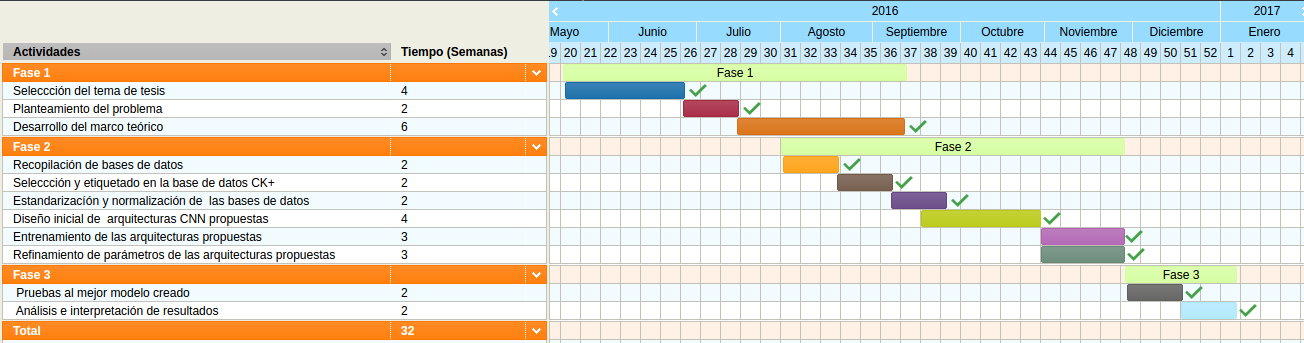
\includegraphics[angle=90,width=60mm]{Imagenes/cronograma.png}
    \caption{Cronograma de actividades}
    \label{tab:tab1}
\end{table}


